\section{Durchführung}
\label{sec:Durchfuehrung}
\begin{figure}
    \centering
    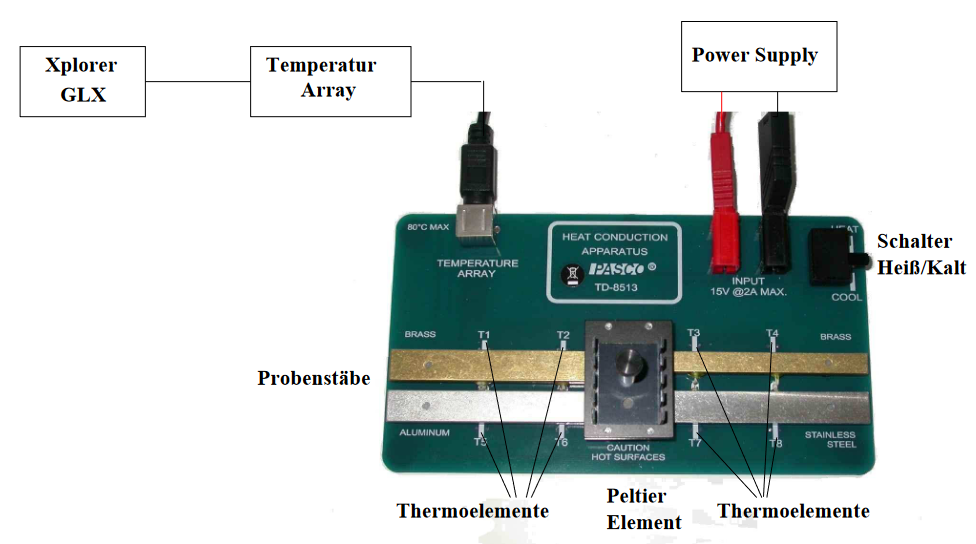
\includegraphics[width=0.7\textwidth]{Versuchaufbau.png}
    \caption{Versuchsaufbau.}
    \label{fig:versuchaufbau}
  \end{figure}

Zur Durchführung des Versuchs, wird der in \autoref{fig:versuchaufbau} gezeigte Versuchsaufbau verwendet, sowie ein Datenlogger zum Aufzeichnen der Temperaturen
T1 bis T8.

\subsection{Statische Methode}
\label{sec:StatischeMethode}

Bei dieser Methode wird bei dem Datenlogger zunächst eine Abtastrate von $\Delta t_{GLX} = 5 \mathrm{\, s}$ eingestellt. Dies bedeutet, dass der Datenlogger alle
5 Sekunden die Temperaturen der 8 Messtellen aufzeichnet. Das Peltier Element wird mit einer Spannung von $U_P = 5 \mathrm{\, V}$ bei maximalen Strom versorgt. \\
Die Wärmeisolierung wird auf die Stäbe gelegt und der Schalter auf "Heiß" gestellt. Die Messung wird so lange durchgeführt, bis das Thermoelement T7 ca. 45 Grad 
Celsius anzeigt. Danach werden die Stäbe so gut wie möglich abgekühlt.\\
Sobald die Metallstäbe kühl genug sind, werden diese wieder erhitzt. Nach etwa 700 s werden die Temperaturen der Messtellen T1, T4, T5 und T8 notiert.

\subsection{Dynamische Methode}
\label{sec:DynamischeMethode} 

Für die Dynamische Methode wird die Abtastrate des Datenloggers auf $\Delta t_{GLX} = 2 \mathrm{\, s}$ eingestellt und die Spannung auf 8 V erhöht. Die Stäbe 
müssen zudem auf mindestens 30 Grad Celsius runtergekühlt sein.\\
Die Stäbe werden nun abwechselnd 40 Sekunden erhitzt und wieder gekühlt, indem der Schalter auf "Heat" und "Cool" gestellt wird. Nach 10 Perioden wird die Messung
abgebrochen und die Stäbe werden wieder abgekühlt.\\
Danach wird dieser Vorgang wiederholt, jedoch werden die Stäbe nun abwechselnd 100 Sekunden erhitzt und wieder gekühlt. Die Messung wird abgebrochen, sobald eins der
Thermoelemente eine Temperatur von 80 Grad Celsius anzeigt. Die Stäbe werden abschließend wieder gekühlt.
\newpage